\section*{Aufgabe 1: \emph{Fisher--Diskriminante: Implementierung}}
\begin{itemize}
\item[a)] Die Mittelwerte der Verteilungen sind: $\vec{\mu_0} = (0.0223003 ; 3.02562461) $ und $\vec{\mu_1} = (5.98570071 ; 3.09798977)$

\item[b)] Die Streumatrix innerhalb der Klassen berechnet sich zu:
\begin{equation}
S_W = 	\begin{pmatrix} 122897.81109658 & 81975.19093279\\
 						81975.19093279 & 67446.72860506
 		\end{pmatrix} 
\end{equation}
Die Streumatrix zwischen den Klassen berechnet sich zu:
\begin{equation}
S_B = 	\begin{pmatrix}	8.89053611e+04  & 1.07885616e+03 \\
						1.07885616e+03  & 1.30917934e+01
 		\end{pmatrix} 
\end{equation}
\item[c)] Die Eigenvektoren berechnen sich zu:
\begin{align*}
\vec{\lambda_1} =& ( 0.63668392 ; -0.77112488 ) \quad \text{mit:}\quad \lambda_1 = 3.71 \\
\vec{\lambda_2} =& ( -0.01213399 ; 0.99992638 ) \quad \text{mit:}\quad \lambda_2 = 1.39 \cdot 10^{-17}
\end{align*}
\item[d)] Die Projektion der Populationen $P_0$ und $P_1$ auf die Geraden $\lambda_i$.
\begin{figure}[H]
	\centering
	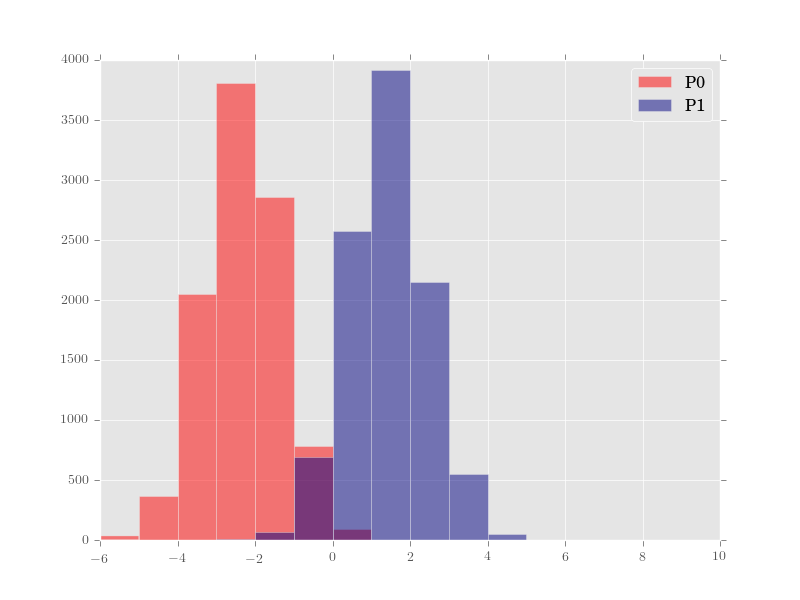
\includegraphics[width=0.7\textwidth]{hist_0.png}
	\caption{ Projektion der Populationen auf die Gerade $\lambda_1$}
\end{figure}
\begin{figure}[H]
	\centering
	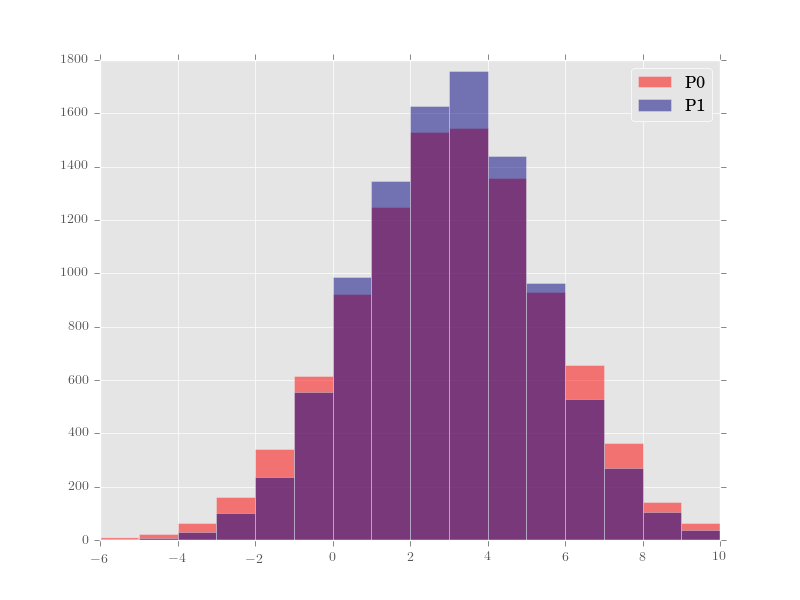
\includegraphics[width=0.7\textwidth]{hist_1.png}
	\caption{Projektion der Populationen auf die Gerade $\lambda_2$}
\end{figure}
\item[e)] Die Performanz in Abhängigkeit des gewählten Schnittes:
\begin{figure}[H]
	\centering
	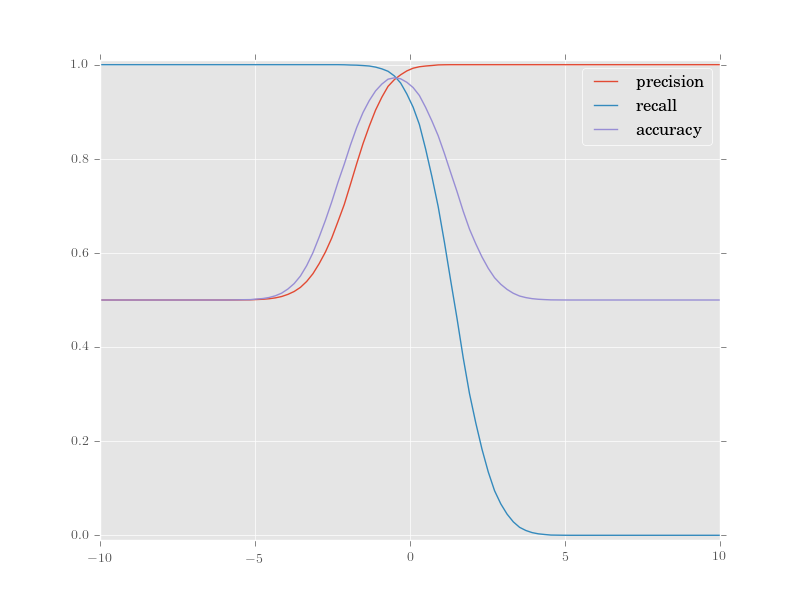
\includegraphics[width=0.7\textwidth]{performace_1.png}
	\caption{Performanz für die Projektion der Populationen auf die Gerade $\lambda_1$}
\end{figure}
\begin{figure}[H]
	\centering
	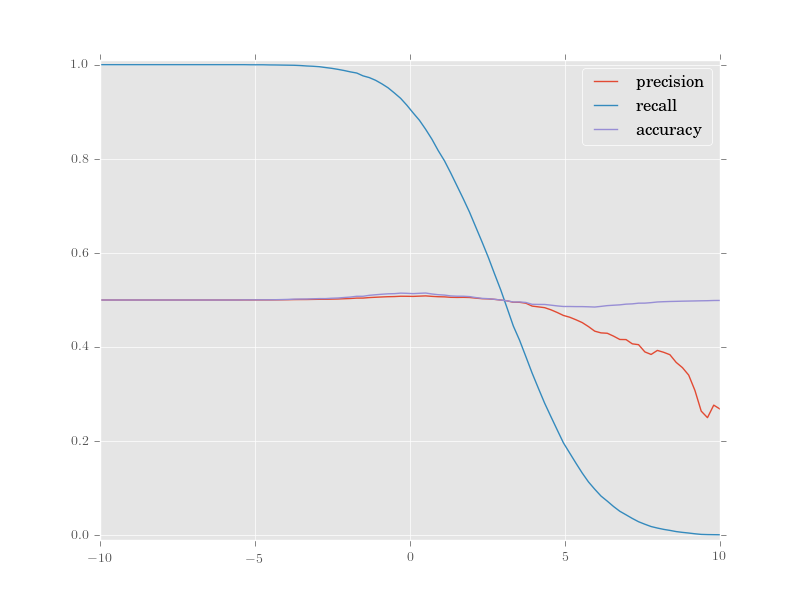
\includegraphics[width=0.7\textwidth]{performace_2.png}
	\caption{Performanz für die Projektion der Populationen auf die Gerade $\lambda_2$}
\end{figure}
\item[f)] Das Signal-Untergrundverhältnis wird für die Projektion auf $\lambda_1$ bei $\lambda_{\text{cut}}\approx -5.76$ und für die Projektion auf $\lambda_2$ bei $\lambda_{\text{cut}}\approx -5.36$ maximal.
\begin{figure}[H]
	\centering
	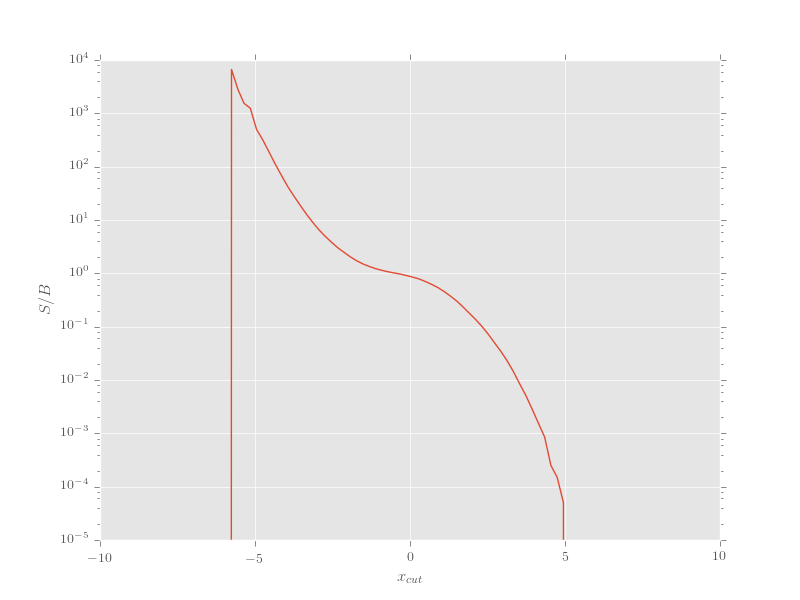
\includegraphics[width=0.7\textwidth]{sig_bkg_ratio.png}
	\caption{Signal-Untergrundverhätnis für die Projektion der Populationen auf die Gerade $\lambda_1$}
\end{figure}
\begin{figure}[H]
	\centering
	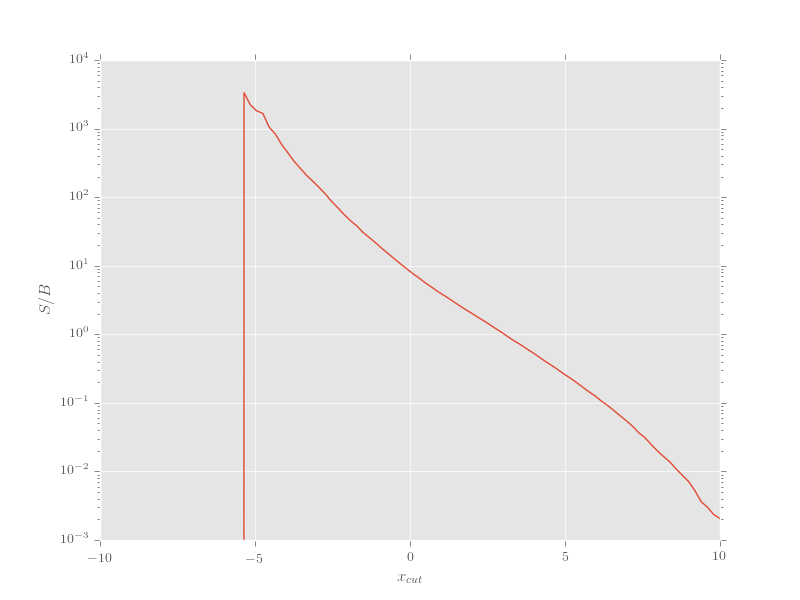
\includegraphics[width=0.7\textwidth]{sig_bkg_ratio2.png}
	\caption{Signal-Untergrundverhätnis für die Projektion der Populationen auf die Gerade $\lambda_2$}
\end{figure}

\item[g)] Die Signifikanz wird für die Projektion auf $\lambda_1$ bei $-10 \leq \lambda_{\text{cut}} \leq -5.96$ und für die Projektion auf $\lambda_2$ bei $-10 \leq \lambda_{\text{cut}} \leq -5.56$ maximal.
\begin{figure}[H]
	\centering
	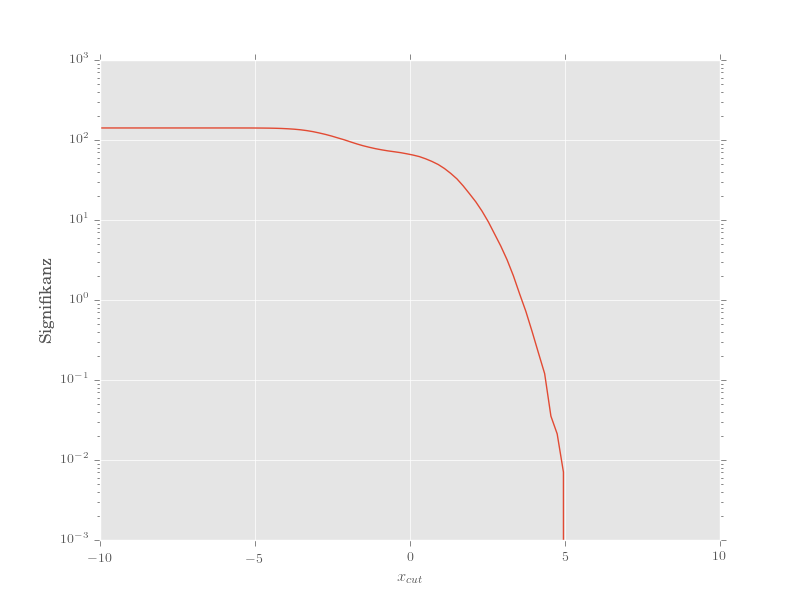
\includegraphics[width=0.7\textwidth]{signifikanz.png}
	\caption{Signifikanz für die Projektion der Populationen auf die Gerade $\lambda_1$}
\end{figure}
\begin{figure}[H]
	\centering
	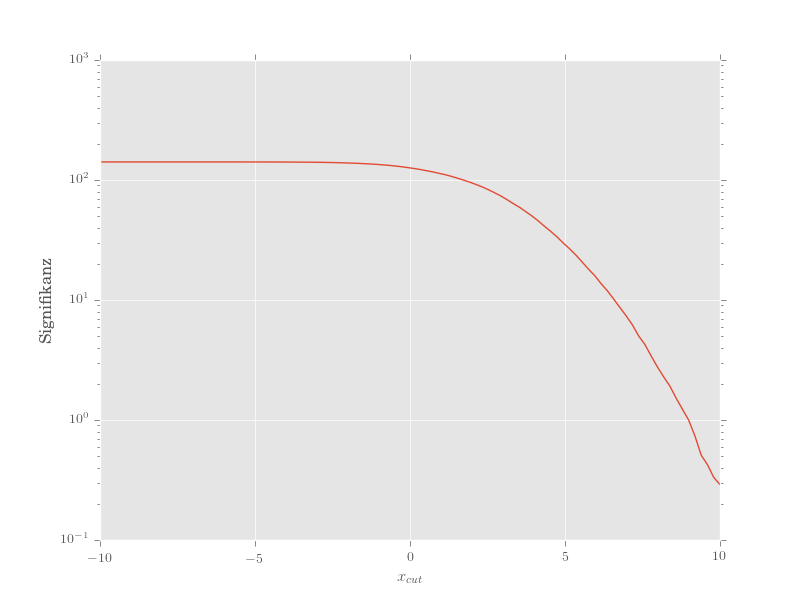
\includegraphics[width=0.7\textwidth]{signifikanz2.png}
	\caption{Signifikanz für die Projektion der Populationen auf die Gerade $\lambda_2$}
\end{figure}

\item[h)] Analog für den kleineren Datensatz von $P_0$ nur mit der Gerade $\lambda_1$.

\item[he)] Die Performanz in Abhängigkeit des gewählten Schnittes:
\begin{figure}[H]
	\centering
	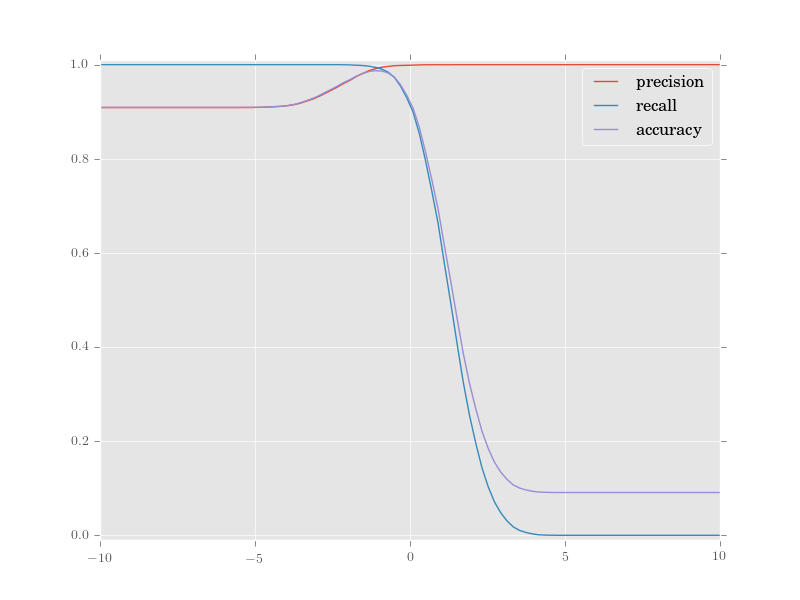
\includegraphics[width=0.7\textwidth]{performace_1_h.png}
	\caption{Performanz für die Projektion der Populationen auf die Gerade $\lambda_1$}
\end{figure}

\item[hf)] Das Signal-Untergrundverhältnis wird für die Projektion auf $\lambda_1$ bei $\lambda_{\text{cut}}\approx -5.35$maximal.
\begin{figure}[H]
	\centering
	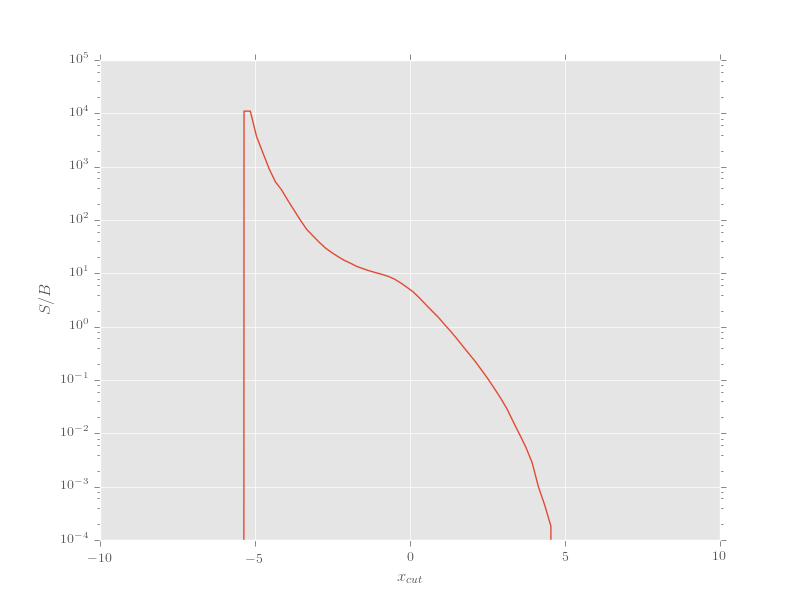
\includegraphics[width=0.7\textwidth]{sig_bkg_ratio_h.png}
	\caption{Signal-Untergrundverhätnis für die Projektion der Populationen auf die Gerade $\lambda_1$}
\end{figure}


\item[hg)] Die Signifikanz wird für die Projektion auf $\lambda_1$ bei $-10 \leq \lambda_{\text{cut}} \leq -5.55$ maximal.
\begin{figure}[H]
	\centering
	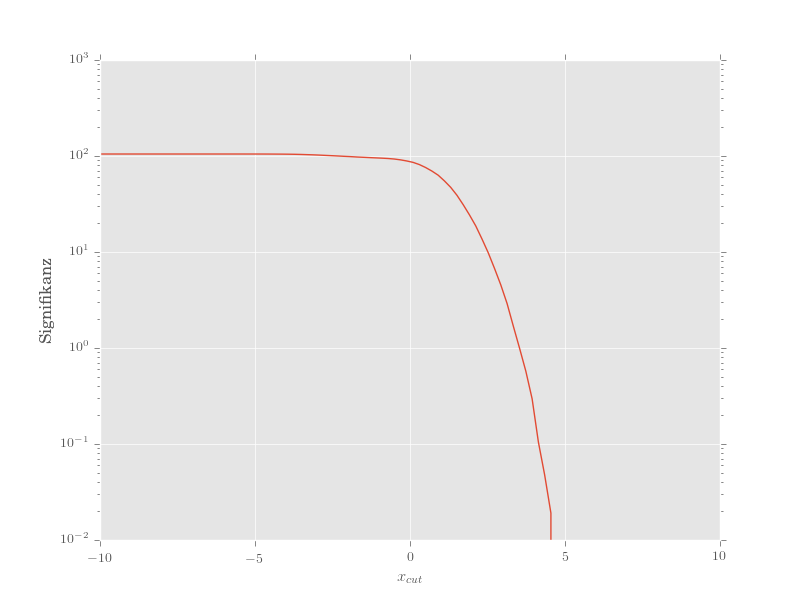
\includegraphics[width=0.7\textwidth]{signifikanz_h.png}
	\caption{Signifikanz für die Projektion der Populationen auf die Gerade $\lambda_1$}
\end{figure}



\end{itemize}
\section*{Aufgabe 2: \emph{kMeans per Hand}}

Population: $(1;4) (1;5) (1;6) (3;3) (3;2) (4;1) (5;1) (6;2) (6;3) (8;4) (8;5) (8;6))$

\begin{itemize}
\item[a)] Clusterzentren $(3;4) (7;4) (3;7)$

\begin{align*}
(3;4): (1;5) (1;4) (3;3) (3;2) (4;1) (5;1)\\
(7;4): (6;2) (6;3) (8;4) (8;5) (8;6) (5;1)\\
(3;7): (1;6)
\end{align*}

\begin{align*}
\text{neue Clusterzentren:}\\
(\frac{17}{6}; \frac{8}{3} ) = (2.83; 2.67)\\
(\frac{41}{6}; \frac{7}{2} ) = (6.83; 3.50)\\
(1; 6 )
\end{align*}


\begin{align*}
\text{neue Clusterzentren:}\\
(\frac{17}{6}; \frac{8}{3} ):(3;2) (3;3) (4;1) (5;1) \\
(\frac{41}{6}; \frac{7}{2} ): (6;2) (6;3) (8;4) (8;5) (8;6) \\
(1; 6 ): (1;4) (1;5) (1;6) 
\end{align*}


\begin{align*}
\text{neue Clusterzentren:}\\
(\frac{15}{4}; \frac{7}{4} ) = (3.75; 1.75)\\
 (7; 2)\\
(1; 5 )
\end{align*}


\begin{align*}
\text{neue Clusterzentren:}\\
(\frac{15}{4}; \frac{7}{4} ):(3;2) (3;3) (4;1) (5;1) \\
 (7; 2): (6;2) (6;3) (8;4) (8;5) (8;6) \\
(1; 5 ): (1;4) (1;5) (1;6) 
\end{align*}

\end{itemize}
\section*{Aufgabe 3: \emph{Feature Selection mit dem MRMR--Algorthmus}}
